\chapter {The Mathematics of Terrain}
\label{chapter:Introduction}

The surface of the Earth is one of the largest and most influential sources of data there is. 
Its shape determines atmospheric conditions, where structures can and should be built, and where flooding is to be expected, for example. 
As such, our quest for full understanding of the physical environment around us relies on an understanding of the underlying mathematics of the Earth's surface.
Therefore terrain data, both surface and volumetric, are vital for a wide array of applications in Computer Graphics and Geographic Information Science (GIS).

% GIS is the discipline charged with collecting, analyzing, and manipulating terrain data. One of the primary challenges in GIS is understanding the underlying mathematics of terrain, and using that understanding to develop more accurate and robust representations of the data that take into account the terrain's hydrography, or behavior of water on the terrain.
% 
This thesis presents a detailed look at terrain modeling through the lens of mathematical analysis, and explores representation and generation of the terrain surface 
through mathematical operations, descriptive statistics, and erosion simulation.




% It presents a method for modeling and representing terrain that is more closely related to the physics of erosion than previous methods based on mathematical operations that
% % , when combined with each other and various parameters, 
% procedurally generate the terrain based on the physical impact of erosion on a terrain surface.
% % , and their mathematical properties are be explored in depth. 
% This model allows for better compression of terrain datasets, as well as a terrain shape that more closely resembles reality than other popular models.
% This work also presents a series of metrics for determining statistical distance between two terrains, including the idea of a terrain "fingerprint", which is a measurement of a series of characteristics based on the terrain's hydrography data.
% %  used to better determine similarity and dissimilarity between terrains and channel networks extracted from those terrains. 
% % These fingerprints lead directly to a method of terrain comparison which determines a "distance" between two terrains, and is used to critically examine the erosion processes that alter the terrain. 
% % Data is collected through the use of a visually-validated and physically based erosion simulation based on smoothed particle hydrodynamics and a model of soil erodibility. This data is processed and allows me to capture snapshots of terrain evolution.
% In addition to modeling the surface with mathematical operations, this thesis presents the work of a research group that has investigated the process of erosion on levee surfaces, and validates the group's results through comparison to laboratory experimentation. 

\section{Modeling Terrain Surfaces}
\label{section:ModelingTerrainSurfaces}

Geographic Information Science is the study, manipulation, collection, management, and analysis of all geographical information, 
blending cartography, modeling, and data analysis and statistics.
One of the primary challenges in GIS is understanding the underlying mathematics of terrain surface data in order to model it accurately, robustly, and compactly.

Between the fields of earth science, computer science, mathematics, physics, and civil engineering, a good deal of work has revolved around modeling terrain surfaces. It is an essential aspect in a variety of applications in GIS, from path planning to dam siting to terrain compression. However, despite the large body of excellent work from which to draw, GIS still lacks a physically realistic representation of terrain that stems from a 
% deep
mathematical understanding of the way in which erosion processes, most specifically hydraulic erosion (the wearing away of a material due to water), contribute to the evolution and formation of a terrain. 
In addition to simply providing for more accurate data, an accurate and compact terrain representation lends itself naturally to better compression schemes, faster algorithms, and more accurate terrain generation. 


The hydrography, or behavior of water, of the terrain is a fundamental property that influences many of the characteristics of the terrain,
% Many applications in GIS (including those presented in this thesis) rely on the hydrography of the terrain, which is represented 
and it governs many of the applications in GIS. 
It is defined by the direction of water flow across the terrain, and allows for the extraction of the channel network (also know as the river or drainage network) of the terrain surface, 
a series of channel segments that join and flow together toward a sink.
Maintaining this critical information should be a primary objective of any terrain representation or generation scheme,
as important applications (such as modeling erosion on earthen embankments, as discussed in Sections \ref{section:ModelingLeveeFailure} and \ref{chapter:ErosionSimulation}) require hydrographically sound terrain representations.


With these goals in mind, this work focuses on the representation and generation of valid terrain, or data that 
% more 
closely mimics real life terrain. Real terrain is not a continuous surface, as discontinuities are common. Cliff faces, the sides of rivers, and caves are all terrain features that introduce discontinuities to any terrain surface representation. 
% Also, local minima (pits, for instance) are hard to find in real terrain, and are often introduced in data as a consequence of inaccuracies in data collection. 
In addition, local minima, or pits, are known to exist in certain terrains, such as those consisting of Karst topography or natural basins (e.g. endorheic basins). 
% \fbox{CITATIONS FOR THEM?}
However, most
local minima present in terrain data are a result of the sampling procedure used to collect it, which may miss channels
that are too small for the spacing of the grid and may
pass between sample points (sometimes called ``posts''). 
Most data collection techniques cannot differentiate between tree cover, lake surfaces, and land, resulting in elevation inaccuracies and pits where there should be none.
% At the scale at which most of these data are collected (with approximately 30 m spacing), local minima should not appear as often as they do. 
One of the principal constraints of any new representation is that it must facilitate the restriction of local minima, especially along the terrain's drainage network, by drawing a connection between the representation and the physics of the terrain's formation.

A method for modeling and representing terrain based on a mathematical operator, the \emph{drill operator}, is presented. This representation is more closely related to the physics of erosion than other purely spatial representations. It also facilitates enforcement of rules to limit the presence of local minima, and allows for discontinuities in the surface to be encoded. 
% than previous methods
 With various parameters, terrain is procedurally and accurately generated. This operator is based on the physical impact of erosion on a terrain surface, and its mathematical properties are explored in depth. 
This model allows for better data compression of terrains, as well as a terrain shape that more closely resembles reality than other popular models.

Current terrain representations are generally variations of either height fields (2D pixel grids of elevations, also known as Digital Elevation Models, or DEMs) or piecewise linear triangular splines (also known as Triangulated Irregular Networks, or TINs). Both of these representations have advantages and disadvantages, but neither sufficiently captures the physical complexity of a terrain surface. For instance, neither can accurately handle discontinuities on the surface, such as cliff faces. 
Each representation is single-valued, meaning that each vertex of data has a unique x,y coordinate. Since the slope of a cliff face is vertical, and as such undefined, any single-valued representation cannot accurately model it.
% 
% TINs are able to, but with added complexity to any algorithm using them, since many applications rely on the grid regularity of the TIN representation. 
Volumetric representations, such as voxel grids, allow for said discontinuities as well as volumetric features such as caves, but have considerable memory footprints, and do not correlate in any way with the geological processes that formed the terrain being represented. 

% \fbox{WTF?}
% A set of procedural steps utilizing a finite set of well-defined drill operators that mimic erosion to form a terrain both saves space and allows for more physically accurate surface features, such as discontinuities and a lack of local minima.

To facilitate the development and testing of the drill operator, a more fundamental understanding of the 
% statistics and characteristics of terrains is necessary. 
% What are the characteristics of terrain necessary to mimic? 
% What are the characteristics of terrain necessary to maintain when compressing it? 
% Part of the answer to these questions lies in the hydrography of the terrain. 
% 
effects and behavior of water on the surface, also known as the terrain's hydrography, is necessary.
This fundamental characteristic can be described by the terrain's channel network, or a series of pixels that describe the flow of water across the surface.
% 
Several methods exist for extracting the channel network,
%(see section \ref{section:PriorLiteratureChannelNetworkExtraction}), 
and much can be done with the information gleaned from it.  
Terrain statistics such as 
% the channel width and depth, 
how much network segments meander, the relative importance of pixels within the network, and the balance of tributaries that join major rivers are measured.
This statistical approach provides a descriptive picture of a terrain that is useful when comparing two terrains (for applications such as measuring compression scheme accuracy), as well as describing the erosion processes responsible for the formation of the terrain.
% Also presented 
This is the \emph{terrain fingerprint}, a series of terrain characteristics used to better determine similarity and dissimilarity between terrains and channel networks extracted from those terrains. These fingerprints lead directly to a method of terrain comparison which determines a metric of distance between two terrains.
% , and is used to critically examine the erosion processes that alter the terrain. 



\begin{figure}[t]
  \centering
  \begin{minipage}{0.99\textwidth}
    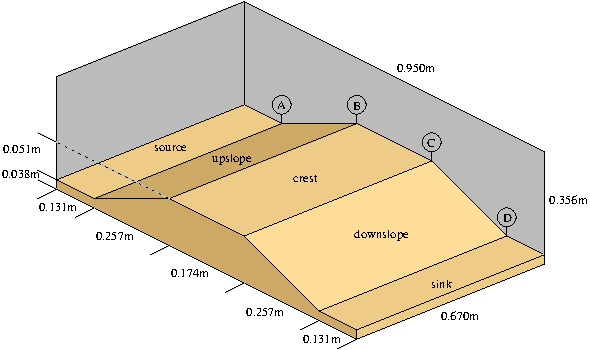
\includegraphics[width=1.0\textwidth]{images/levee_diagram.pdf}
  \end{minipage}
  \caption[Annotated diagram of a levee]{An annotated diagram of a levee, detailing the wet side (source, upslope), crest, and dry side (downslope, sink). Measurements refer to those of model levees created in a laboratory for experimentation.}
  \label{figure:levee_diagram}
\end{figure}



\section{Modeling Levee Failure}
\label{section:ModelingLeveeFailure}

\begin{figure}[t]
  \centering
  \begin{minipage}{0.49\textwidth}
    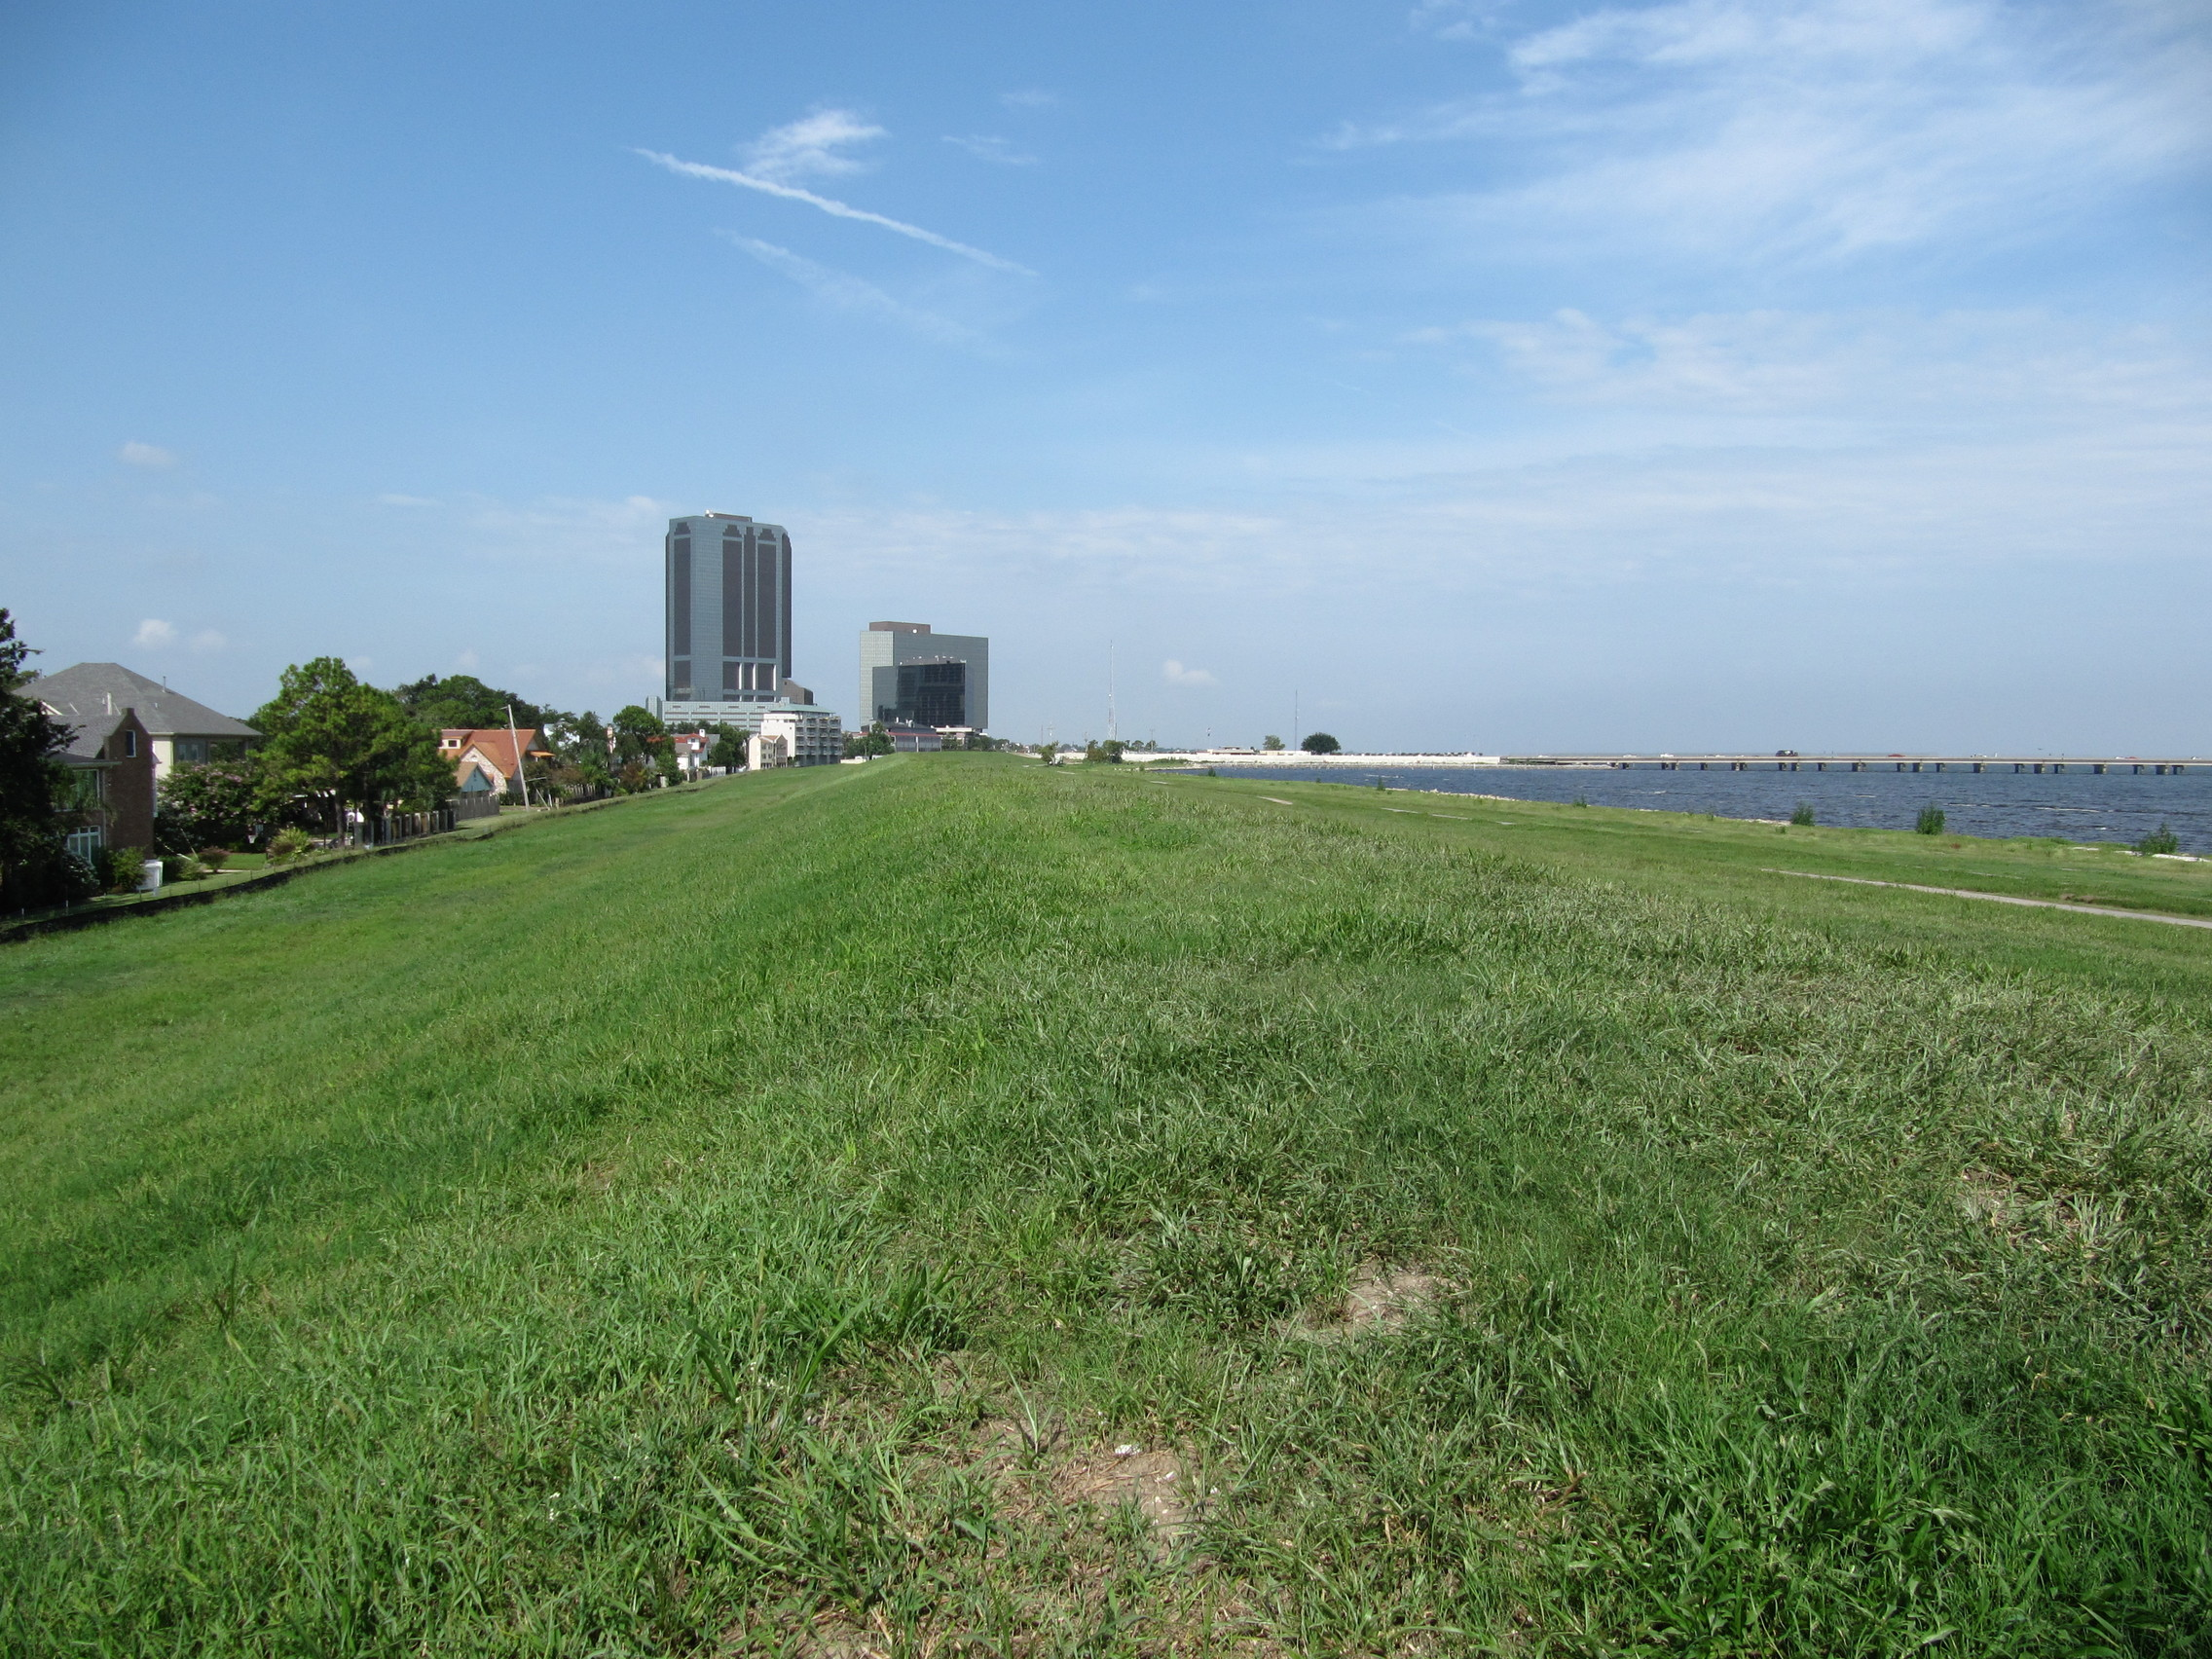
\includegraphics[width=1.0\textwidth]{images/GrassyLakeLevee.jpg}
  \end{minipage}
  \begin{minipage}{0.49\textwidth}
    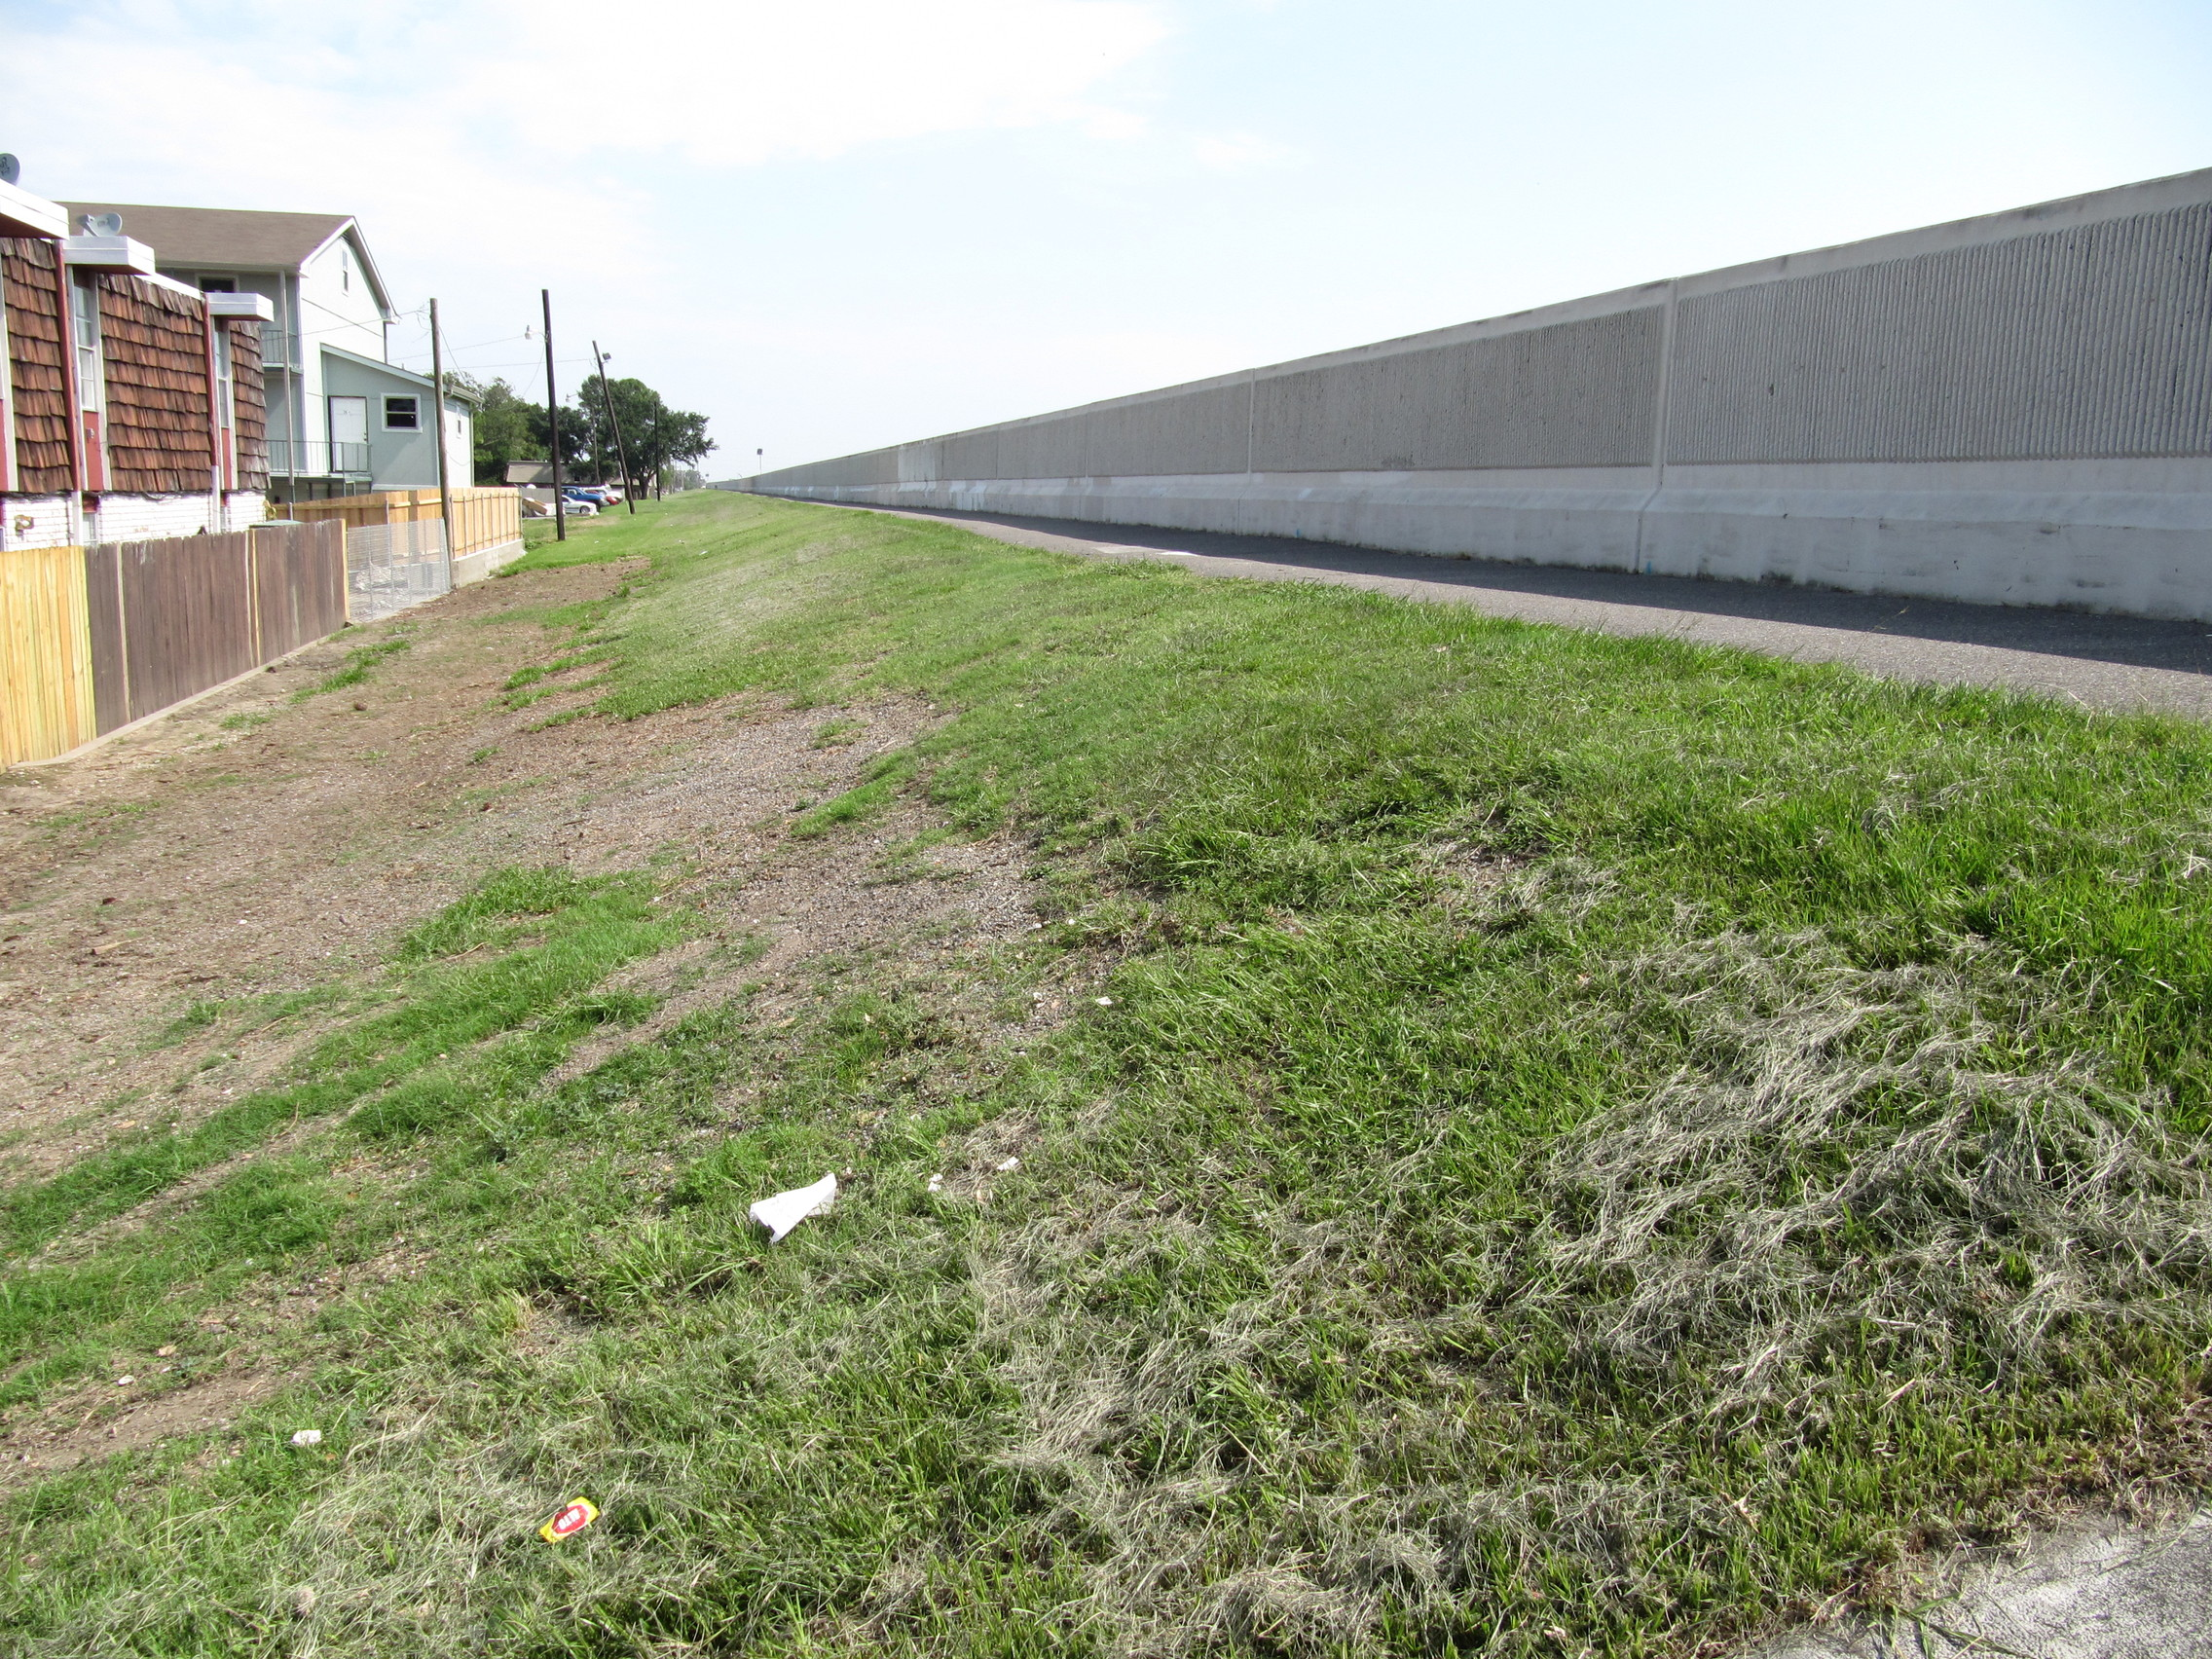
\includegraphics[width=1.0\textwidth]{images/DryLeveeWithRetainingWall.jpg}
  \end{minipage}
    \caption[Levees in New Orleans, LA]{(Left) An earthen lake levee in New Orleans, LA. (Right) An earthen levee with a temporary cement wall protecting a residential neighborhood in New Orleans, LA.}
    \label{figure:levees}
\end{figure}



\begin{figure}[t]
  \centering
  \begin{minipage}{0.99\textwidth}
    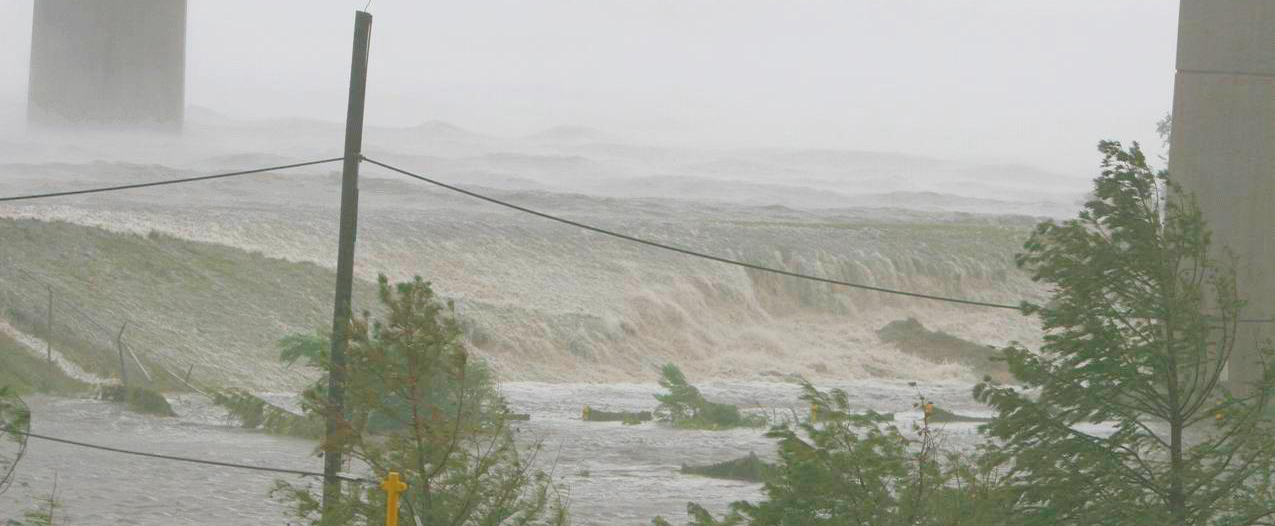
\includegraphics[width=1.0\textwidth]{images/zimmie_Picture2b_crop.jpg}
  \end{minipage}

  \begin{minipage}{0.99\textwidth}
    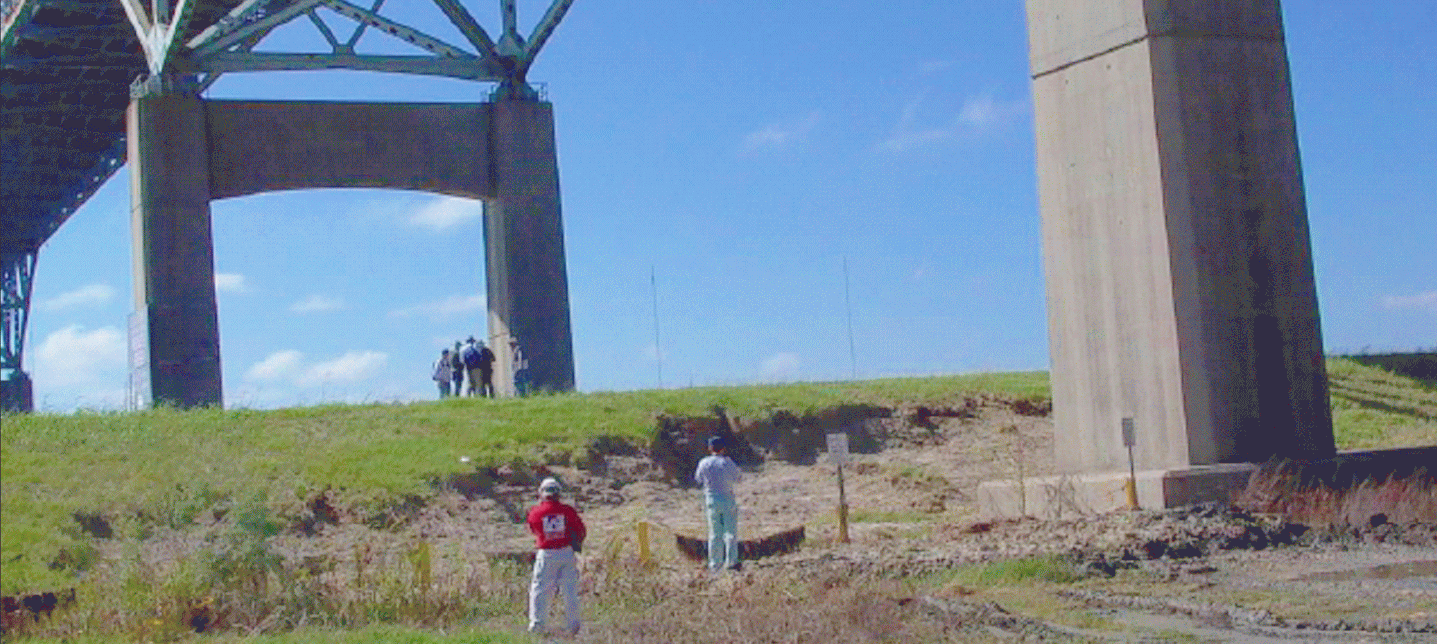
\includegraphics[width=1.0\textwidth]{images/zimmie_Picture1b_crop.png}
  \end{minipage}
  \caption[An overtopped levee]{A levee that was overtopped for several hours during
    Hurricane Katrina but did not fail.  The dramatic gouging/scooping
    on the lower portions of the levee is due to increased waterflow at
    the base of the levee and the non-homogeneous nature of the
    embankment.}
  \label{figure:katrina_photos}
\end{figure}



\begin{figure}[t]
  \centering
  \begin{minipage}{0.99\textwidth}
    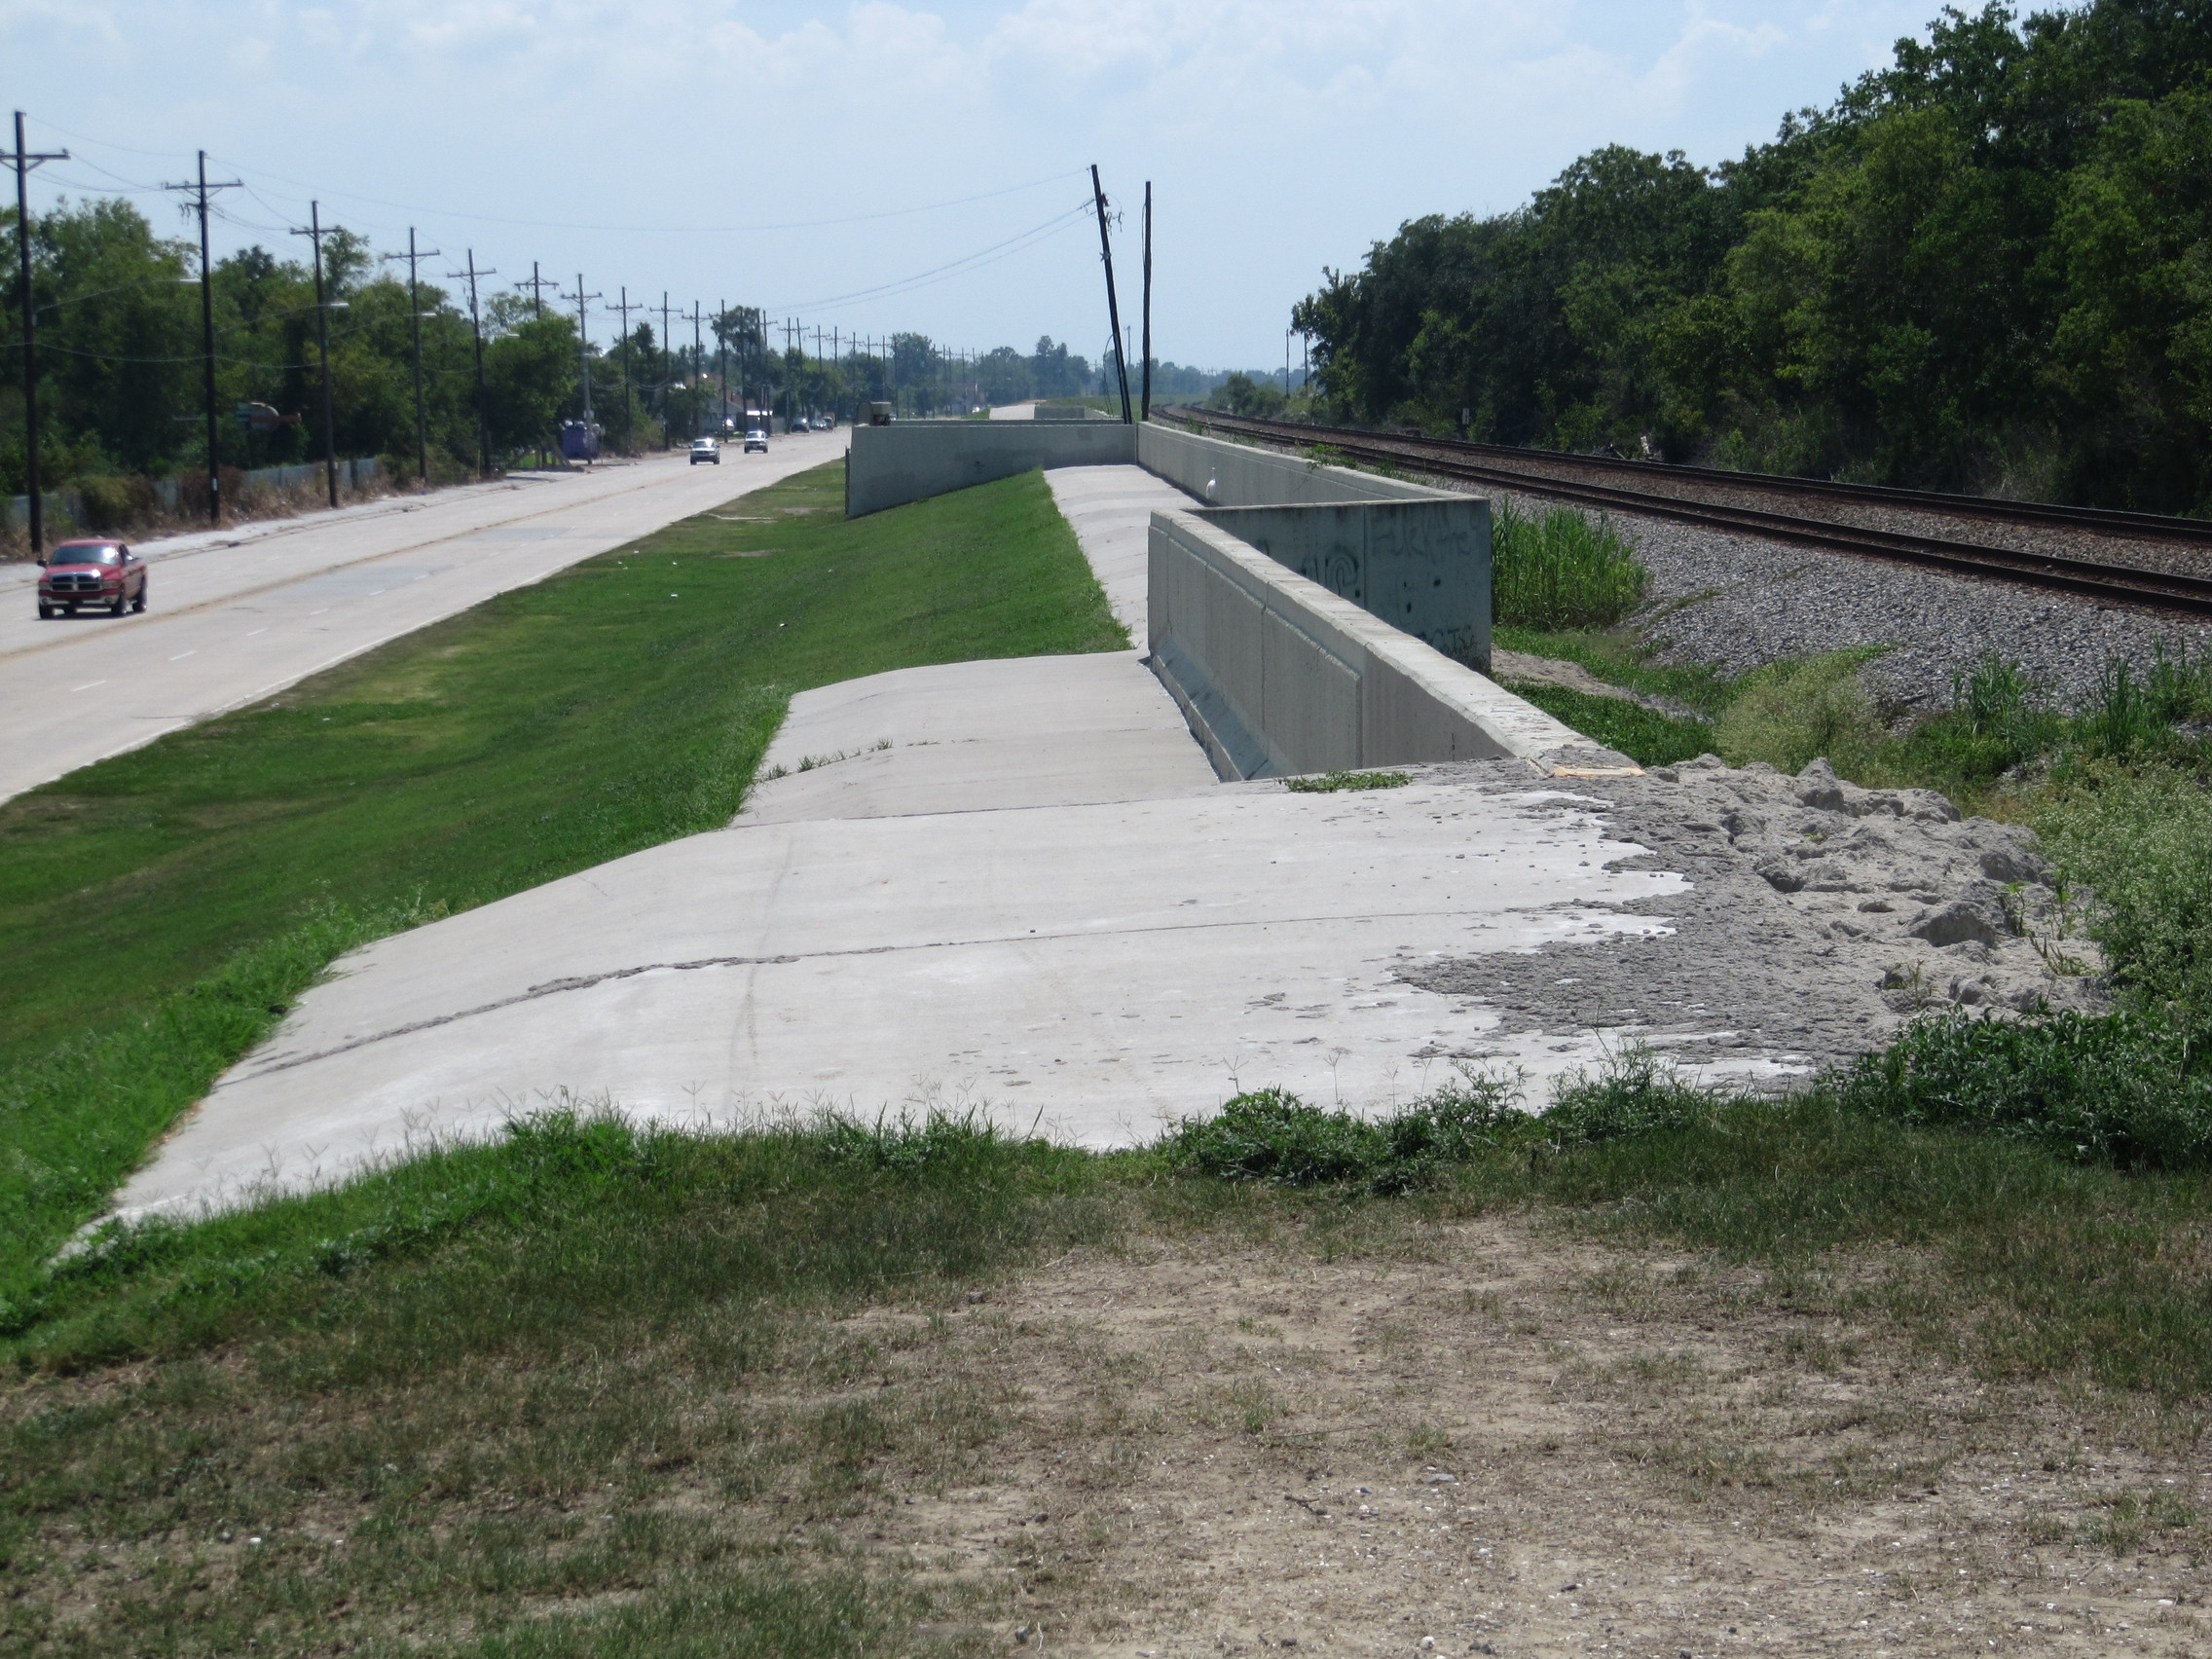
\includegraphics[width=1.0\textwidth]{images/RebuiltLevee.jpg}
  \end{minipage}
  \caption[A replacement cement wall]{A levee that failed during Hurricane Katrina and has been replaced with a temporary cement wall.}
  \label{figure:rebuilt_levee}
\end{figure}



% An understanding of the evolution of terrains makes possible the process of simulating it and, eventually, simulating its reverse.
% 
% A primary benefit of a deeper understanding of the evolution of terrain is the ability to simulate the reversal of the process. 
Given an original terrain and an eroded terrain, the ability to identify the series of operations on the original that formed the final eroded one is an interesting and challenging problem. One application of this forensic analysis is diagnosing earthen embankment (specifically levee) failure due to erosion, a primary motivation for this work.

Erosion in this thesis refers to hydraulic erosion, or the physical wearing away or breaking down of a material, usually a soil, by running water. 
% Other types of erosion include glacial and wind erosion. 
An earthen embankment is a sloped piece of land that is made 
% entirely 
of earthen materials, such as sand or clay. Earthen dams are walls of earthen material that hold a body of water over a long period of time, whereas earthen levees are two-sided embankments that protect objects on one side against periodic rising waters and crashing waves from the other (Figure \ref{figure:levee_diagram}). Some levees have non-earthen components, such as retaining walls or cores, made of less erodible materials like wood or clay. Some are replaced by cheaper materials, such as cement (Figure \ref{figure:levees}).
% , which is a hard (often cement) wall protruding from the top of it, or a core made of less erodible material, such as clay. 

Levee breach is the process whereby a channel through a levee forms due to high soil volume loss from hydraulic erosion, allowing water to pour through. Once breach has occurred, the failure of the levee is imminent. The time of breach is usually defined as the moment when the headcut (the very edge of the eroded channel) reaches point C in Figure \ref{figure:levee_diagram}, where the crest and the downslope meet. At this moment, an erosion channel that had been making its way across the crest widens and becomes a freeway for waterflow.
Levee breach and failure are most often caused by overtopping, the occurrence of water flowing over the crest of the levee, usually caused by high waves during a storm surge.

There are other methods for protecting levees against failure. Planting grass on the levee surface slows the rate at which erosion cuts channels in it. Levees can also fail by a process known as piping, or internal (subsurface) erosion, caused by water permeating the surface and eroding away the levee's foundation. A clay core works to mitigate this process, as does the use of geosynthetic materials through the body of the levee.

After a
catastrophe involving levee breach, such as the tragedy in New Orleans
during Hurricane Katrina, civil engineers attempt to piece together
the causes of the failure, usually seepage and/or
overtopping \cite{SENATE_REPORT} (Figure \ref{figure:katrina_photos}). 
% 
% \fbox{DEFINE OVERTOPPING}
% 
Forensic analysis of the cause of these failures is becoming more and more critical in assessing levee construction and safety, and its automation
makes this necessary process
more accessible.
%  faster and cheaper. 
% 
In addition, studying the erosion process that causes this failure in depth, including the formation of breach channels, the velocity and behavior of water, and the rate of the breach event, can lead to better levee construction and modeling, and is a primary motivation for the general purpose modeling problem presented in Section \ref{section:ModelingTerrainSurfaces}. A better understanding of the formation of the terrain surface and a better model for it go hand-in-hand.


Historically, there are many examples of levee failures, such as those by levees surrounding New Orleans during Hurricane Katrina (Figure \ref{figure:rebuilt_levee}).  Perhaps one of the most famous failures of an embankment dam by overtopping was the 1889 Johnstown, PA dam failure which killed more than 2000 people, left thousands homeless, and transformed the prospering city of Johnstown into a virtual wasteland \cite{Schnitter}.  Numerous other examples can be cited, but it is clear that such failures can cause serious loss of lives and economic disaster. Also, flood damage in the US cost \$50,000,000,000 in the 1990s \cite{FloodDamageData}. 
This largely unnecessary loss of money and lives can be mitigated with more detailed and accurate methods for studying and analyzing levee failures.
% Better understanding the ways in which earthen structures that are designed to help protect against flooding fail is an important step toward preventing this largely unnecessary loss of money and lives.
Erosion is such a fundamental and devastating natural process that representing terrain data by mimicking it is essential. One attempt to do so, using the drill operator, is presented in Chapter \ref{chapter:DrillOperator}.
% One which facilitates the study and analysis of erosion of levees leading to their failure involves the formation of a detailed hydraulic erosion simulation.


This thesis presents, in part, the work of a research group aiming to automate the diagnostic process of levee failure analysis by performing a detailed study of the levee geometry.
% , represented as one or more DEMs.


\begin{figure}[t]
  \centering
  \begin{minipage}{0.99\textwidth}
    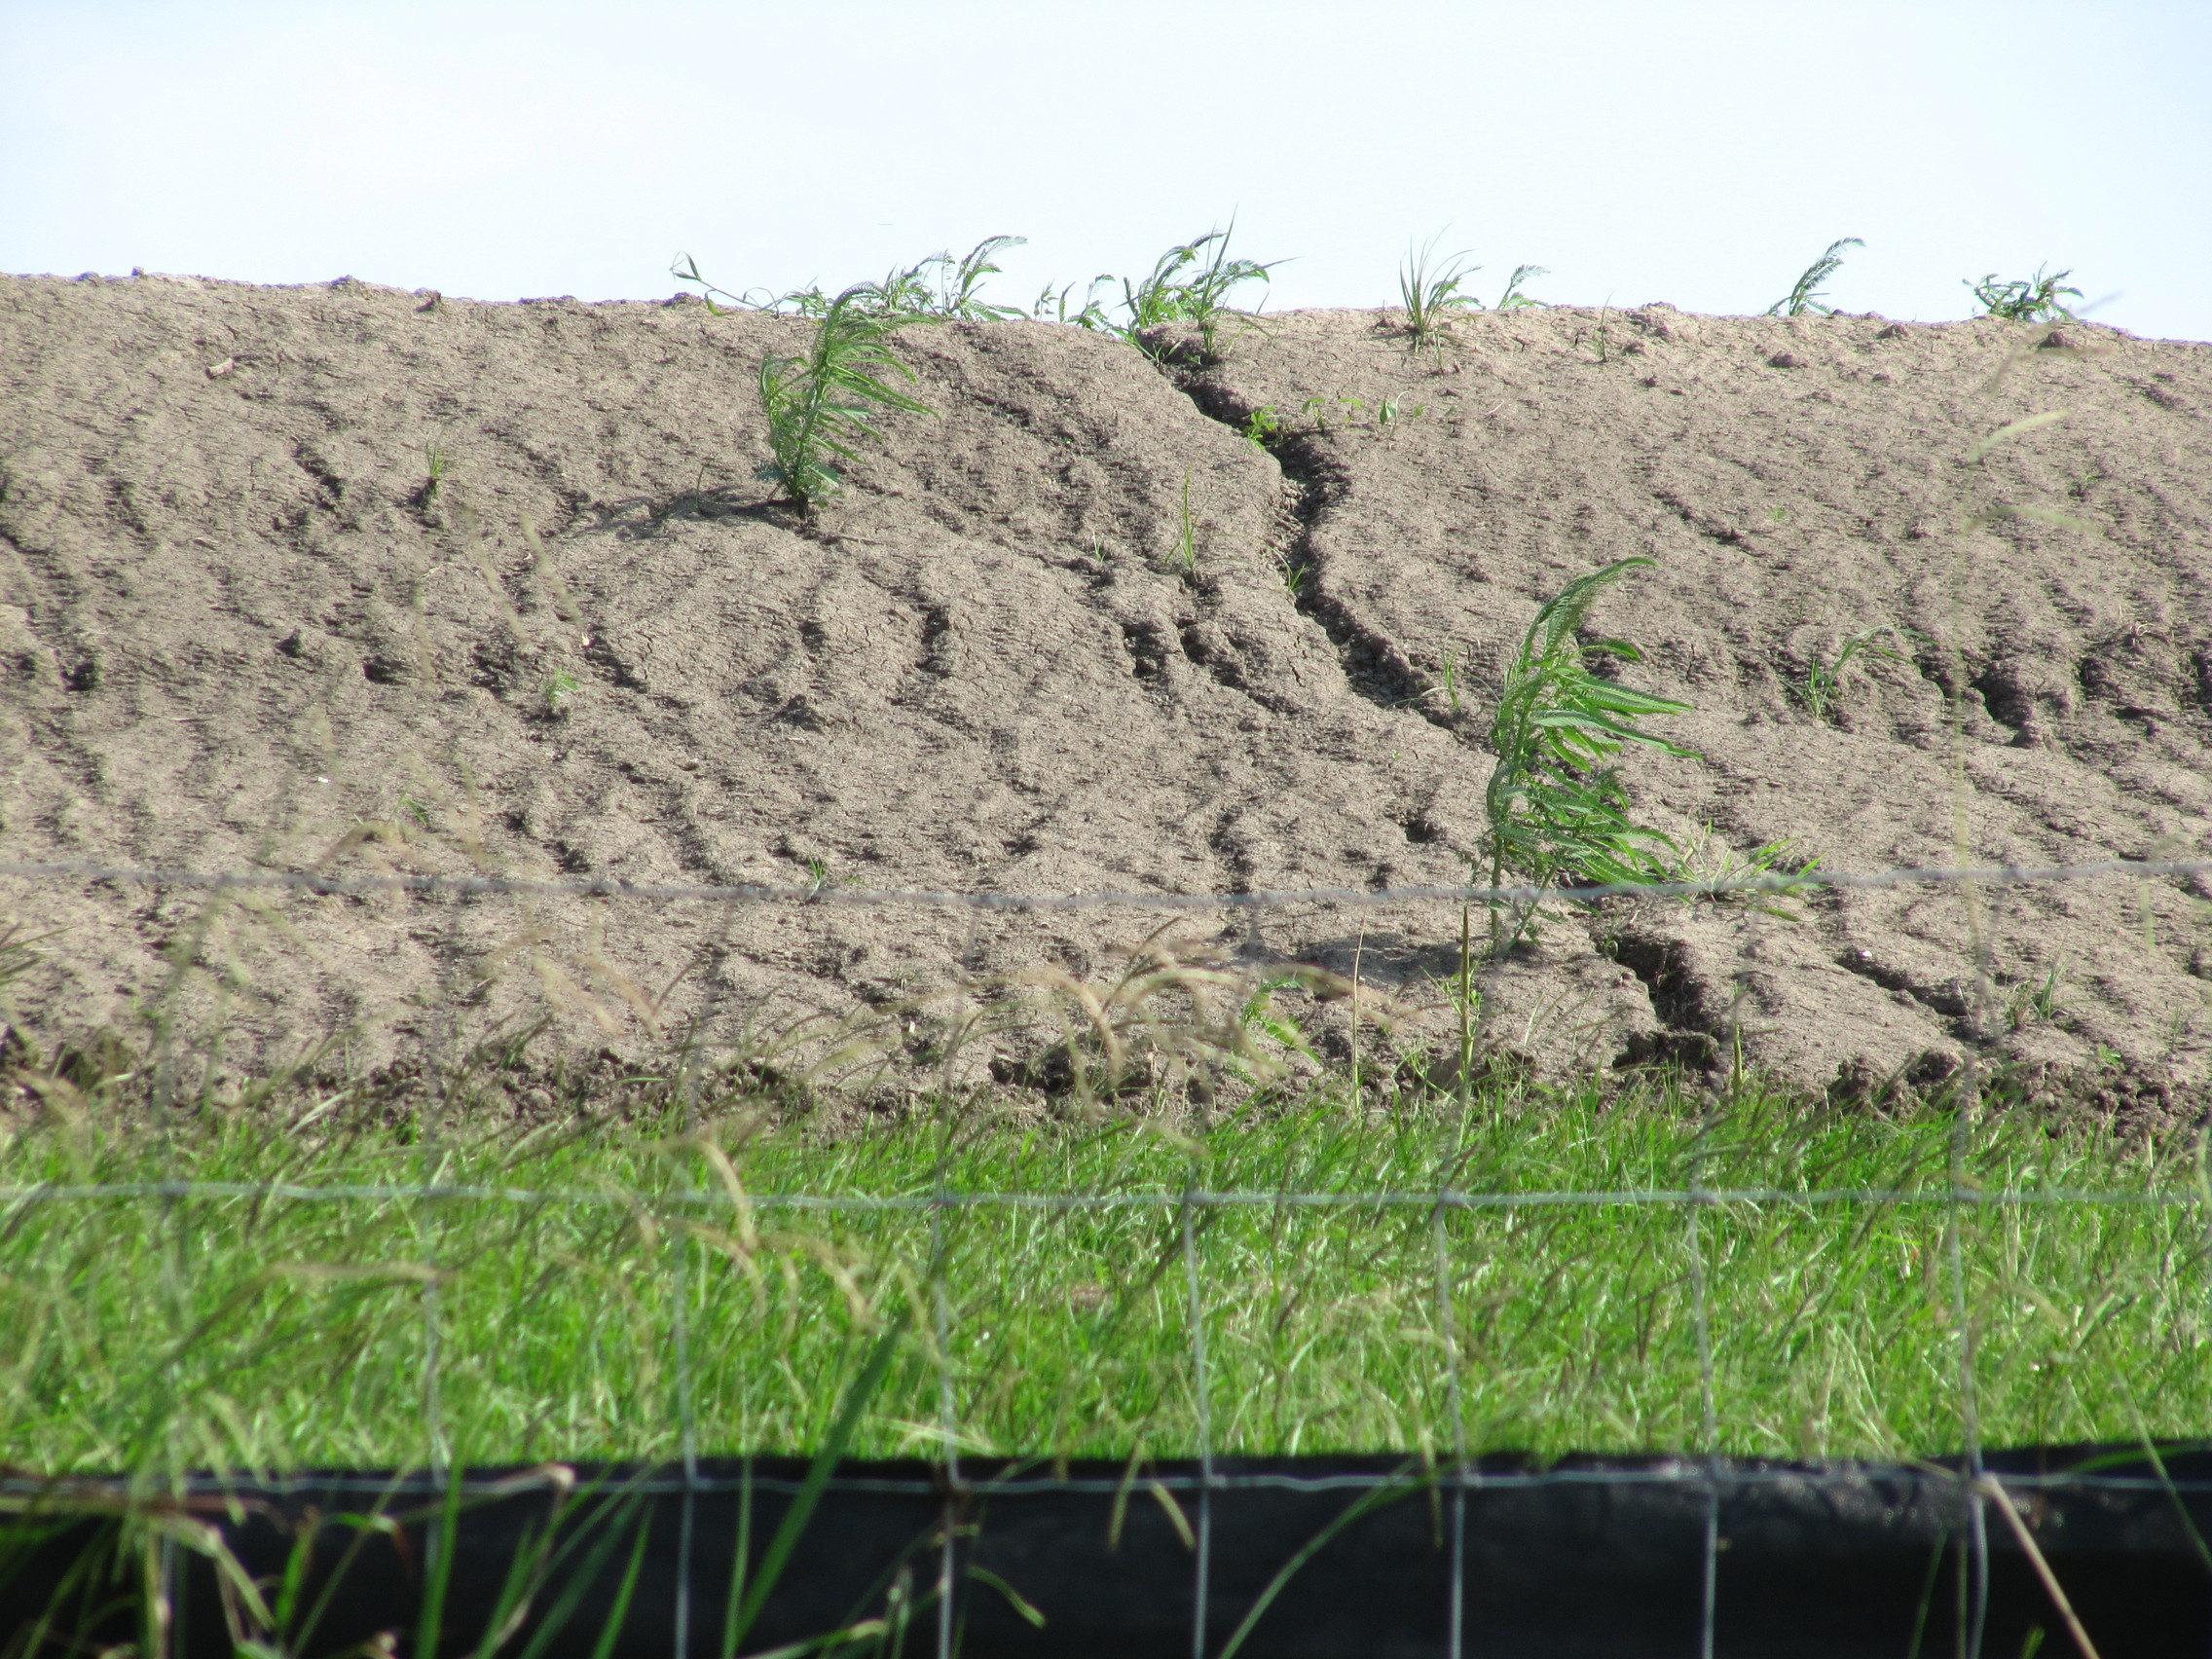
\includegraphics[width=1.0\textwidth]{images/RillsAndGullies.jpg}
  \end{minipage}
  \caption[Eroded channels on an earthen embankment]{An earthen embankment with eroded channels dug out of it.}
  \label{figure:rills_and_gullies}	
\end{figure}



This research focuses on small-scale erosion, which causes rills and gullies to form in the embankment (Figure \ref{figure:rills_and_gullies}). 
% During hydraulic erosion, other formations may develop in the soil, such as a head-cut, which is a sudden sharp cliff in the soil. 
% This formation erodes as a waterfall does as water runs over it. 
To study this, laboratory erosion experiments have been conducted at both 1-g and high-g levels (where ``g'' stands for gravitational units, or -9.8 $\dfrac{m}{s^2}$) in which a small-scale levee is constructed out of 
% Nevada 
sand and water is run over it.
% (figure \ref{figure:1GExperiments}). 
Results are recorded and the geometry of the surface of the levee, both before and after the experiment, is collected for comparison to simulation results. 
% scanned with a LIDAR scanner for use as input to our group's erosion simulation.
%  (chapter \ref{section:ErosionSimulation}).

The group's primary goal has been the development of a detailed and accurate erosion simulation that models laboratory experiments of levee failure. 
Erosion is simulated on an initial levee geometry using Smoothed Particle Hydrodynamics (SPH), coupled with a hydraulic erosion model well-known in civil engineering literature, the erodibility index model. This simulation is validated using analysis of the geometry of the laboratory experiments, both visually and statistically. This thesis presents an analysis of these results.

% In order for automated forensic analysis of levee failures to be a reality, a method must exist for measuring the changes between before and after geometry of the levee surface that goes beyond simple elevation changes. 
% Toward this goal, a framework has been developed for
% % Toward this goal, I have developed a framework for
% detailed comparison of eroded terrains that introduces the notion of
% terrain distance, a measure of how dissimilar two terrain datasets are.
% Methods for measuring terrain distance using the terrain's fingerprint, as well as the general spatial and hydrographic properties of the terrain, are introduced in this thesis. This framework is used to judge the overall accuracy of the group's results, the accuracy of the drill operator representation, and methods for determining the optimal channel network, while taking into consideration only the most important characteristics of the terrain surface.
% % combining channel network and terrain characteristic
% % distance metrics. This set of characteristics is the terrain \emph{fingerprint} (chapter \ref{section:FingerprintingATerrain}), and it governs a series of metrics that measure the dissimilarity between the drainage networks of two terrains (chapter \ref{section:DissimilaryMetrics}).

% MOVE THIS TO THE SIMULATION SECTION!!!!!

% \begin{figure}[t]
%   \centering
%   \begin{minipage}{0.98\linewidth}
%   \begin{minipage}{0.355\textwidth}
%     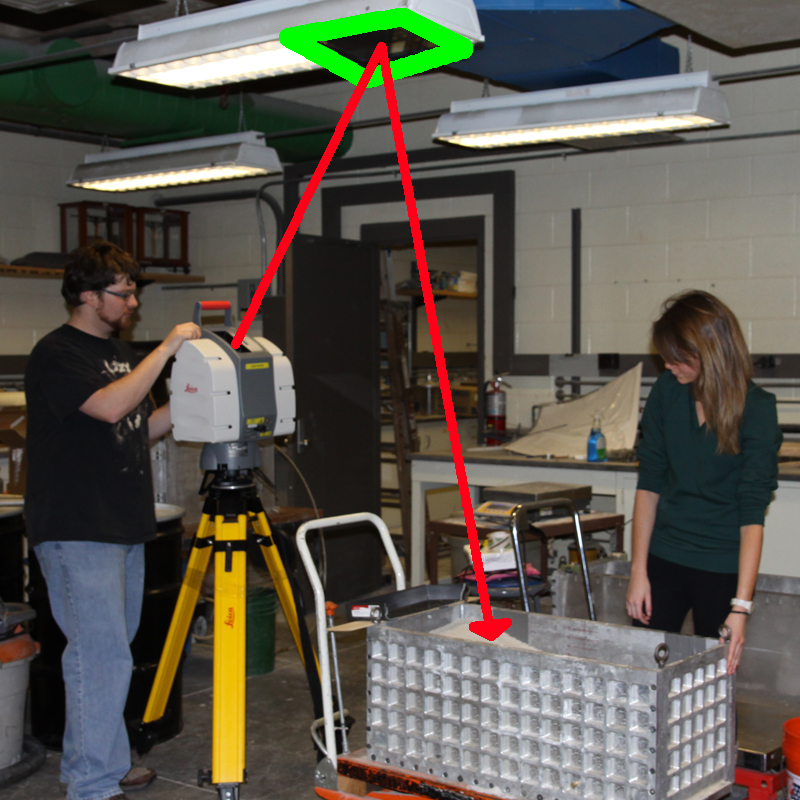
\includegraphics[width=\textwidth]{images/scanner_setup_small_annotated.jpg}
%   \end{minipage}
%   \begin{minipage}{0.635\textwidth}
%     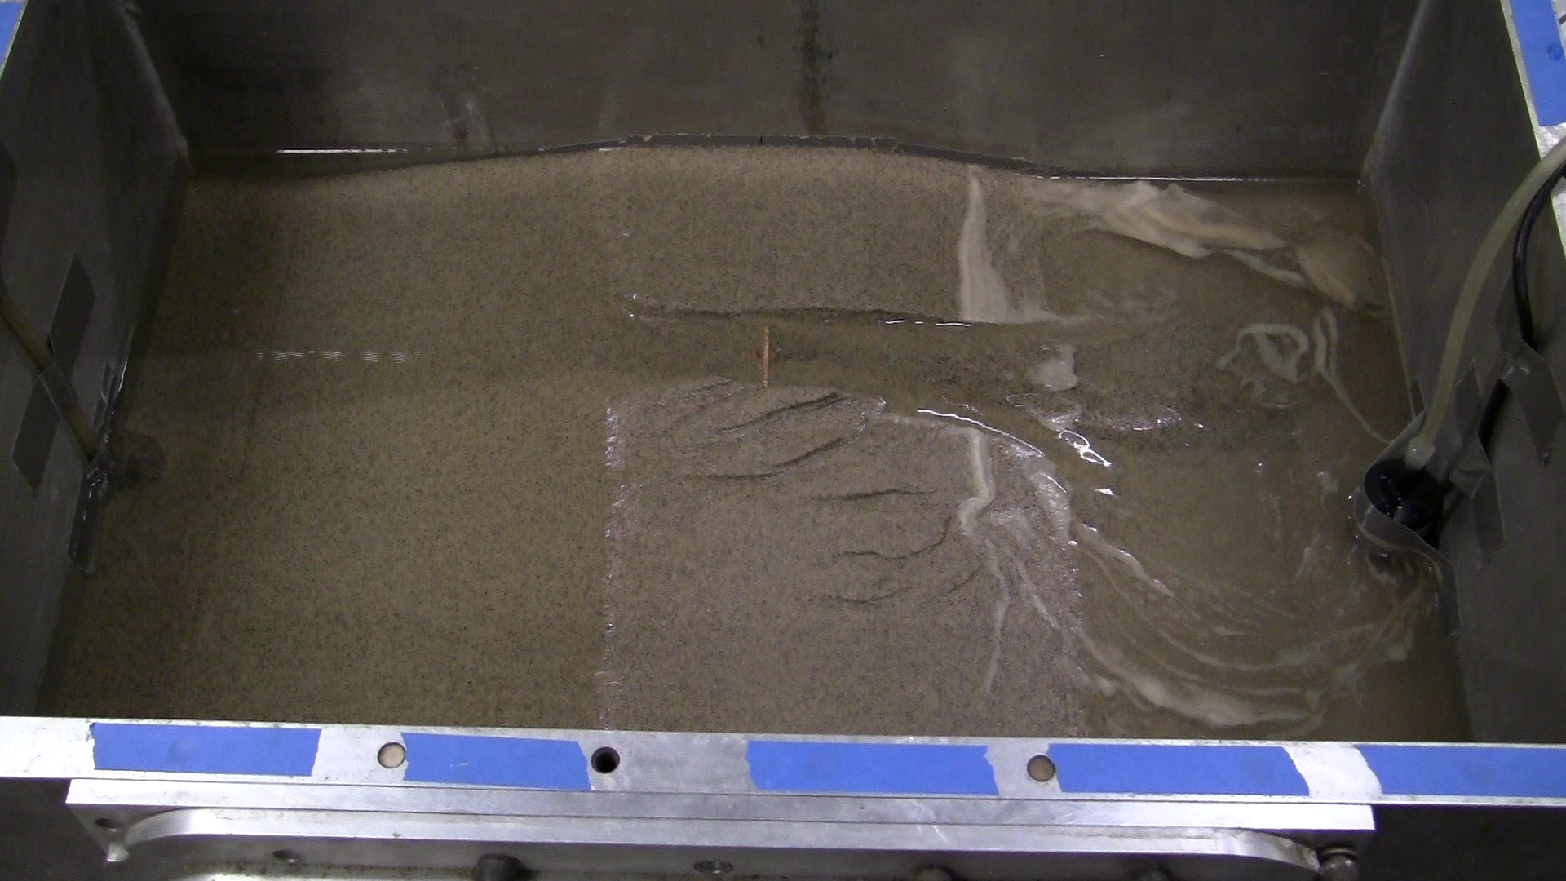
\includegraphics[width=\textwidth]{images/sand-10mins-phy-test.png}
%   \end{minipage}
%   \end{minipage}
%   \caption[Experimental setup of real world experiments]{\label{figure:1GExperiments} Left: LIDAR scanner setup, where LIDAR beams are shot off of a mirror placed on the ceiling and hit the surface of the levee model. Right: An image from the 1-g experiment, in which water flows left to right. A deep channel has clearly formed along the down slope of the levee model.}
% \end{figure}

\section{Data Manipulation and Exploration}

Spatial datasets are more useful if there exist methods for their exploration and manipulation. This thesis presents a system for large-scale group interactive problem solving using inexpensive, off-the-shelf laser pointers for this purpose. It is an example of an application with broad impact and utility that uses the models and simulation presented in Sections \ref{section:ModelingTerrainSurfaces} and \ref{section:ModelingLeveeFailure} for the educational purpose of allowing users to explore terrain data and view how slight changes in elevation values can have a strong impact on the behavior of water on the terrain.
% 
With this system, groups can, using an inexpensive and easy set-up, interactively explore terrain and hydrography data. The system allows each laser pointer to be uniquely identified among its peers by taking advantage of the fact that many inexpensive lasers leak infrared light as they do not include effective IR filtering. 

Since it is possible to uniquely identify each laser pointer, the system can be used for multi-user problem solving and data exploration. This work presents an application that displays an input terrain surface and allows the users to explore the data in a variety of ways. The system allows many users to each select their own individual actions using a button-based user interface. These actions include moving the camera, dropping rain on the surface, and manipulating elevation values along the surface of the terrain. The interactive-time nature of the application allows users to make changes to the terrain and see how the hydrography is effected immediately.

% Also presented in this work is a series of other applications using this technology, including games and emergency response programs.

\section{Contributions and Outline of Thesis}

% \fbox{THIS SECTION WILL BE DOUBLE CHECKED LATER}

This thesis presents the following contributions:

\begin{enumerate}
  \item The \emph{drill operator}, which mimics the process of drilling out a section of the terrain
%   \begin{enumerate}
%     \item An investigation of the effect of various drill shapes on the accuracy of the drill representation
    \item A compression scheme based on the \emph{drill operator} and an analysis of its compression ratios and accuracy
%     \item A method for post-processing terrain data to increase accuracy of \emph{drill operator}.
%     \item A method for \emph{machining} the terrain, applying finer and finer drills to the surface.
%   \end{enumerate}
%   \item A set of distance metrics that allow for the comparison of terrains
  \item The identification of various characteristics of a terrain surface, called the terrain's \emph{fingerprint}, that allow for comparison and analysis of terrain data
%   \begin{enumerate}
%     \item Channel width and depth fields
%     \item Channel meander field
%     \item Junction balance field
%     \item Pixel load field (intuitively, measure of importance of pixel)
%   \end{enumerate}
  \item An application of the Earth Mover's Distance to the probability distributions created by the fingerprint, allowing for measuring terrain dissimilarities
  \item A method of weighting terrain pixels when extracting the drainage network
%   \item A method for selecting a threshold for channel network extraction that allows for closer correlation between the channel networks of sequential terrains
  \item The segmented height field (SHF), a data structure designed for the volumetric representation of layered soil models
  \item A method for tetrahedralizing the SHF to form a closed tetra mesh for rendering and conversion to an SPH grid
%   \item A pipeline for capturing terrain surface data in a laboratory environment and converting it to the SHF
  \item Examination of the results from a series of erosion simulations on levee models
  \item A system for collaborative group interaction for data exploration on a large scale display using laser pointers
  \item A data exploration and manipulation educational application using the laser pointer system to explore and manipulate terrain surface data for educational purposes
\end{enumerate}


% \fbox{THIS NEEDS TO BE UPDATED}
This document is organized as follows: Chapter \ref{chapter:DrillOperator} presents the hydrography channel network extraction method used in this work, and a new representation of the terrain surface, the drill operator.
To determine the accuracy of the drill operator, several metrics for measuring terrain dataset distances are discussed.
Also presented is a compression scheme using this new representation, and a discussion regarding future directions of the drill operator.
Chapter \ref{chapter:FingerprintingATerrain} presents a definition and description of the terrain fingerprint, including the hydrographical characteristics that make it up, and its use in conjunction with the Earth Mover's Distance as a measure of dissimilarity between datasets.
Chapter \ref{chapter:ErosionSimulation} presents the results of several laboratory experiments modeling erosion on a levee surface, as well as the details of an accurate simulation of erosion using SPH, including an analysis of results.
Finally, Chapter \ref{chapter:TerrainDataExploration} presents a system for exploring and manipulating terrain data in a large-scale group-based setting, an application of the work in this thesis focused on its educational prospects. 
Chapter \ref{chapter:ConclusionAndDiscussion} draws a series of conclusions drawn from the work in this thesis, and a discussion of various applications of this work.


% , and its applications of it are presented in Chapter \ref{chapter:UsingTheDrillOperator}. Chapter \ref{chapter:TerrainDistances} introduces several metrics for measuring the distance between two terrain datasets, and Chapter \ref{chapter:FingerprintingATerrain} presents a definition and description of the terrain fingerprint. Chapters \ref{chapter:ErosionModeling} presents the results of several laboratory experiments modeling erosion on a levee surface, and Chapter \ref{chapter:ErosionSimulation} presents the details of an accurate simulation of erosion using SPH, including an analysis of results. Finally, Chapter \ref{chapter:TerrainDataExploration} presents a system for exploring and manipulating terrain data in a large-scale group-based setting, an application of the work in this thesis focused on its educational prospects. Chapter \ref{chapter:ConclusionAndDiscussion} wraps up with a series of conclusions drawn from the work in this thesis, and a discussion of ways in which this work can be extended.
